\chapter{Факторы, влияющие на разрешение литографии}
\section{Формирование пучка в электронном микроскопе}

Электронно-оптическая система электронного микроскопа конструируется таким образом, чтобы получать минимально возможный размер пучка электронов, при этом учитывая максимально возможной ток. На рисунке~\ref{fig:1}. представлена общая схема электронного микроскопа

\begin{figure}[H]
\center
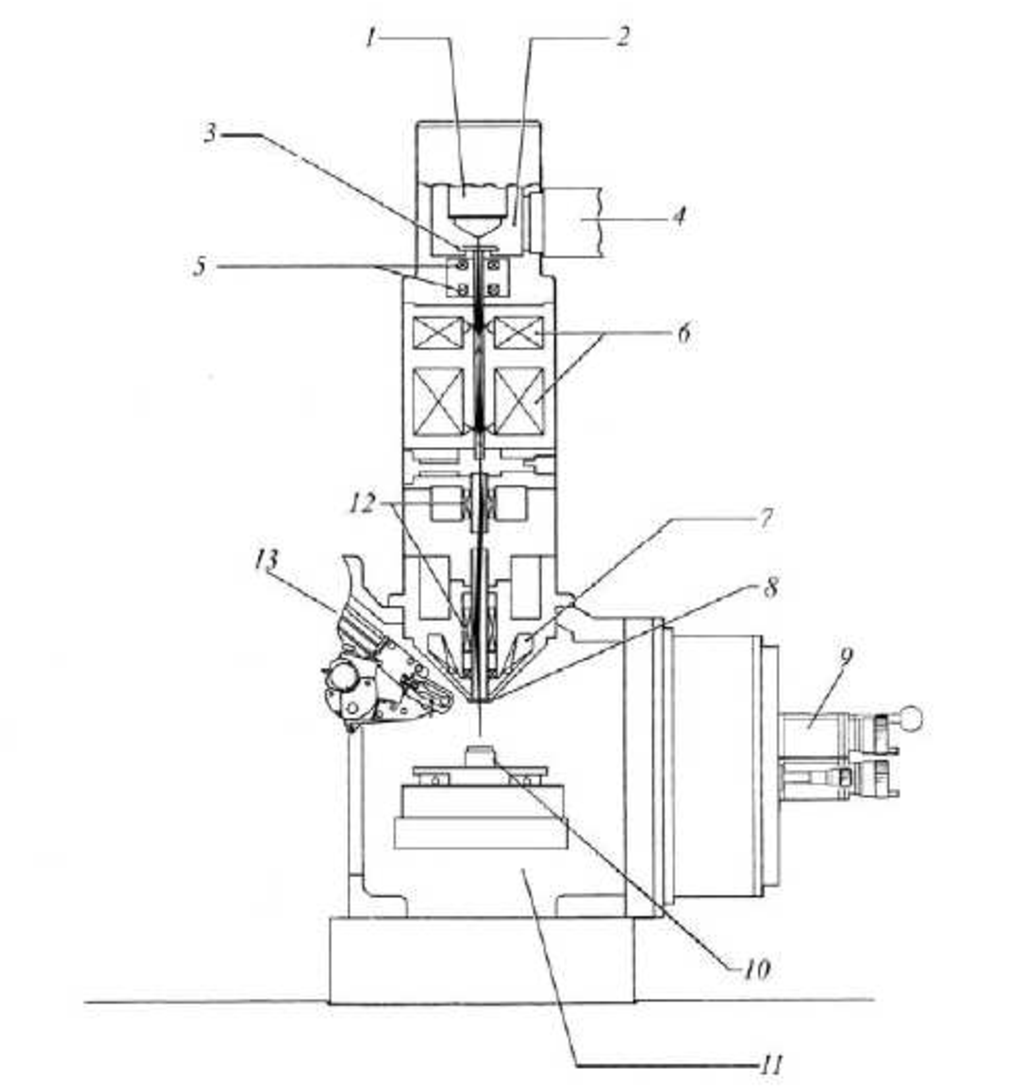
\includegraphics[scale=0.6]{1_1.pdf}
\caption{Общая схема сканирующего электронного микроскопа: 1~--~электронная пушка; 2~--~камера электронной пушки; 3~--~анод; 4~--~вакуумная магистраль; 5~--~котировочные катушки; 6~--~конденсорные линзы; 7~--~объектная линза; 8~--~детектор упруго отраженных электронов; 9~--~система позиционирования образцов; 10~--~держатель образцов; 11~--~основная вакуумная камера; 12~--~сканирующие катушки; 13~--~рентгеновский спектрометр.}
\label{fig:1}
\end{figure}

Электронная пушка является стабильным источником электронов и используется для формирования электронного пучка. На рисунке~\ref{fig:2} представлена общая схема электронной пушки на вольфрамовом катоде.

\begin{figure}[H]
\center
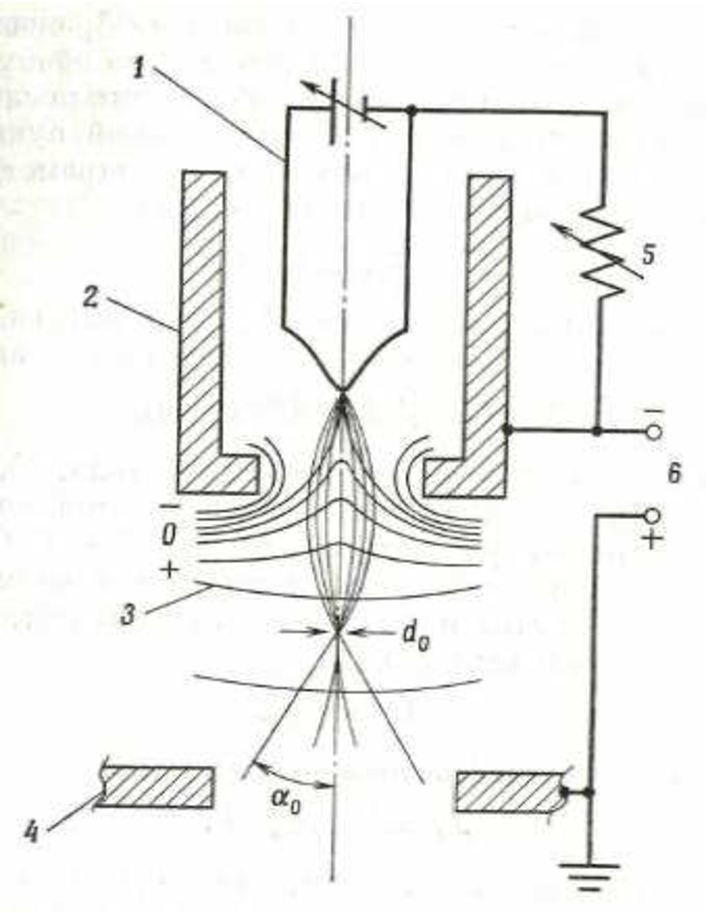
\includegraphics[scale=0.6]{1_2.pdf}
\caption{Схематическое изображение электронной пушки и траектории электронов в ней: 1~--~катод, 2~--~модулятор (цилиндр Венельта), 3~--~эквипотенциали, 4~--~анод, 5~--~сопротивление смещения, 6~--~источник высокого напряжения. $\alpha_0, d_0$~--~угол расхождения электронов и диаметр.}
\label{fig:2}
\end{figure}

Катод, цилиндр Венельта и анод образуют трехэлектродную пушку. В пространстве между цилиндром Венельта и анодом пучок сужается, образуя кроссовер.
Диаметр кроссовера определяется тепловым разбросом скоростей и фокусным расстоянием пушки:
\begin{equation}
d_c \approx 2f \sqrt{\frac{kT_k}{eV_a}}.
\label{eq:A1}
\end{equation}

Важной характеристикой электронной пушки является яркость. Она определяется как плотность тока в единице телесного угла:
\begin{equation}
\beta = \frac{\Delta I}{\Delta S\Delta\Sigma}= \frac{i}{\pi \alpha^2}= \mathrm{const}.
\label{eq:A2}
\end{equation}
Яркость остается постоянной для всех точек на оси электронно-оптической системы от катода до конечного пятна пучка независимо от диафрагм и электронных линз в электронной оптике. Теоретически достижимое значение яркости:
\begin{equation}
\beta_{max} \simeq \frac{i_c E}{\pi kT_c}.
\label{eq:A3}
\end{equation}

На рисунке~\ref{fig:3} схематически представлена электронно-оптическая система, которая создает уменьшенное изображение кроссовера.
\begin{figure}[H]
\center
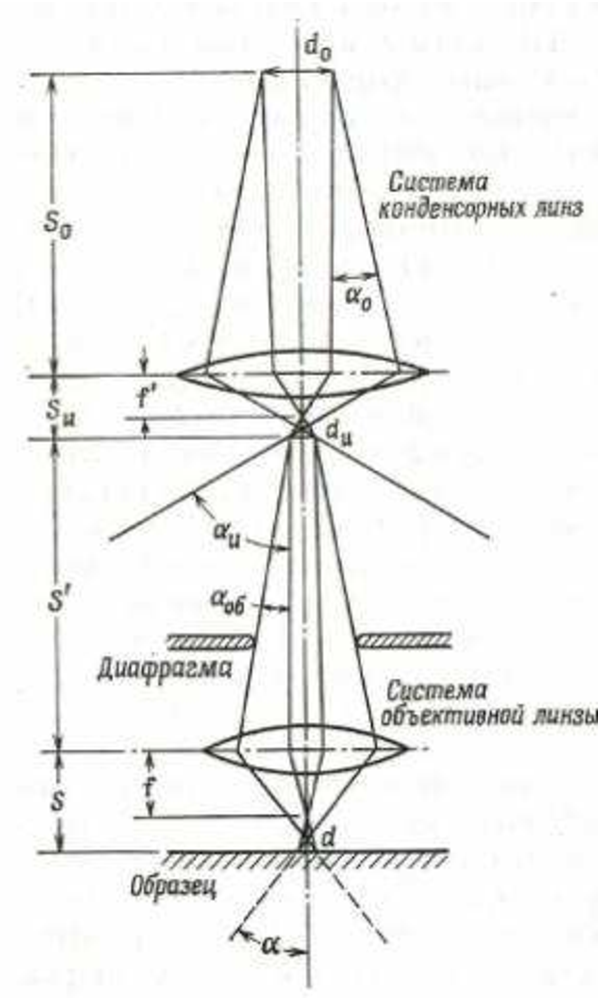
\includegraphics[scale=0.6]{1_3.pdf}
\caption{Схематический ход лучей в электронно-оптической колонне типичного электронного микроскопа.}
\label{fig:3}
\end{figure}

В случае идеальной оптической системы получение пучка минимального размера ограничивалось бы получением уменьшенного изображения кроссовера. Но, в реальных системах имеют место факторы, приводящие к уширениям минимального размера, такие как аберрации, астигматизм и дифракция.

Сферические аберрации дают уширение

\begin{figure}
    \center
    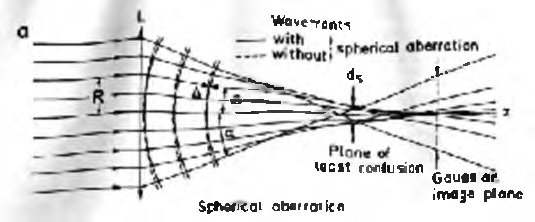
\includegraphics[width=.75\textwidth]{A.pdf}
    \parbox[t]{.95\textwidth}{\centering{а)}}
    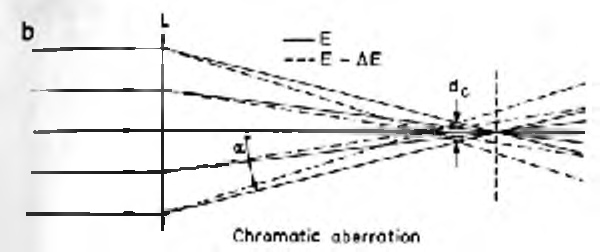
\includegraphics[width=.75\textwidth]{B.pdf}
    \parbox[t]{.95\textwidth}{\centering{б)}}
    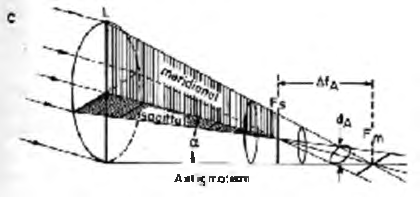
\includegraphics[width=.75\textwidth]{C.pdf}
    \parbox[t]{.95\textwidth}{\centering{в)}}
    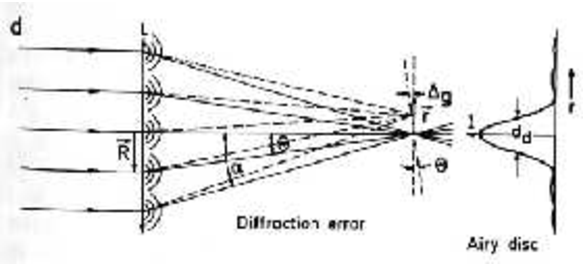
\includegraphics[width=.75\textwidth]{D.pdf}
    \parbox[t]{.95\textwidth}{\centering{г)}}
    \caption{Факторы, приводящие к уширениям минимального размера}
\end{figure}

Для устранения этих эффектов используются электронные линзы специальной конфигурации.
Формирование конечного пятна происходит последовательным уменьшением кроссовера в 2-3 электронных линзах:
\begin{equation}
d_0= \frac{f_1 f_2 f_3}{L_1 L_2 L_3} d_c = md_c.
\label{eq:A4}
\end{equation}
Эффективный диаметр конечного электронного пятна задается
\begin{equation}
d_p^2=d_0^2+d_d^2+d_s^2+d_c^2.
\label{eq:A5}
\end{equation}
Слагаемыми ответственными за дифракцию и хроматическую аберрацию можно пренебречь ввиду их малости. Таким образом, решая задачу по определению наилучшего соотношения размера конечного пучка электронов к току, получается
\begin{equation}
\alpha_{opt}\sim\left(C_0/C_s\right)^{1/4},\>\>d_{p,min}\sim\left(C_0^3 C_s\right)^{1/4},\>\> I_{p,max}\sim \beta C_s^{-2/3} d_{p,min}^{8/3}.\label{eq:A6}
\end{equation}
Здесь
\[
    d_0= \left(\frac{4I_p}{\pi^2 \beta}\right)^{1/2} \alpha_p^{-1}=C_0\alpha_p^{-1},
    \quad j_p=\pi \beta \alpha_p^2 , I_p= \frac{\pi d_0^2 j_p}{4}.
\]

Таким образом, при неизменном токе
\begin{equation}
d_{p,min}\sim (eU)^{-3/8},d_{p,min}\sim(eU)^{-1/2};
\label{eq:A7}
\end{equation}
в идеальной оптической системе
\begin{equation}
d_{p,min}\sim (eU)^{-3/8},d_{p,min}\sim(eU)^{-1/2}.
\end{equation}

\section{Рассеяние электронов и эффекты близости}

Основной проблемой электронной литографии является эффект близости, который заключается в рассеянии электронов в резисте и подложке и экспонировании ими резиста. На рисунке~\ref{fig:4} представлены траектории рассеяния электронов в резиста на кремниевой подложке для энергий 10 кВ и 20 кВ, полученные результат моделирования методом Монте-Карло в работе \cite{4}

\begin{figure}[H]
\center
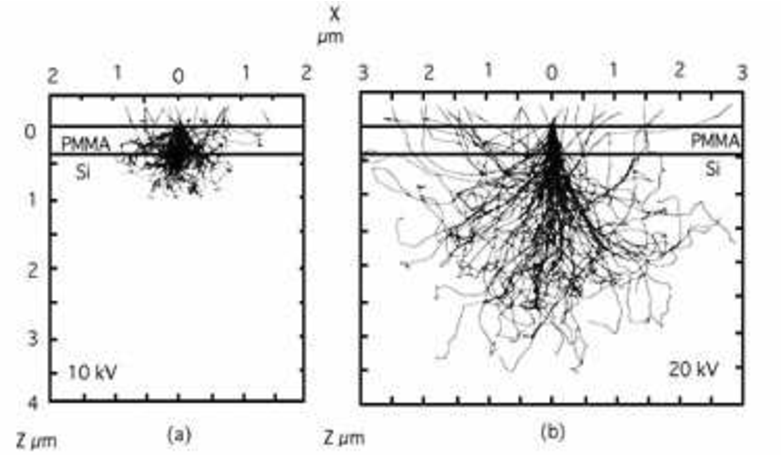
\includegraphics[scale=0.6]{1_4.pdf}
\caption{ Расчет траекторий рассеяния электронов в пленке резиста на кремниевой подложке, выполненный методом Монте-Карло, для энергии электронов 10кВ (слева) и 20кВ (справа)}
\label{fig:4}
\end{figure}

Как видно из рисунка~\ref{fig:4}, область экспонирования обратно рассеянными электронами гораздо больше диаметра электронного луча и составляет микроны, зависит от ускоряющего напряжения и от типа подложки. Длина пробега при рассеянии пропорциональна $E^{1.7}$, где Е- энергия электронов в падающем луче
В зависимости от отсутствия или наличия ближайших соседей наблюдается соответственно внутренний или взаимный эффект близости . Внутренний эффект близости, обусловленный обратным рассеянием электронов за

пределы непосредственно экспонированной области, приводит к тому, что уединенные мелкие элементы топологии проявляются гораздо медленнее, чем большие фигуры. Взаимный эффект близости заключается в экспонировании ближайшими соседями друг друга и пространства между ними. Неэкспонированные области между линиями засвечиваются обратно рассеянными электронами.
Эффект близости в электронной литографии количественно описывается функцией близости
Функция близости~-- это распределение энергии (дозы) экспонирования, поглощенной в резисте. Она является суммой двух гауссовых функций, описывающих вклады в поглощенную дозу первичных электронов
Для решения проблемы коррекции эффекта близости используются несколько способов. Наиболее распространенным способом является коррекция дозы экспонирования. Доза экспонирования каждого элемента структуры устанавливается с учетом влияния эффекта близости так, чтобы в результате проявления все элементы структуры проявились одновременно и с точными размерами.

Эффект близости в электронной литографии количественно описывается функцией близости

% эта формула слишком широкая пусть будет ы 2 этажа снизу спросто и по центру вторая формула пусть будет
\begin{gather}
I(\rho)=\frac{I_1 (\rho)+ \eta I_2(\rho)}{1+\eta}=\frac{1}{\pi(1+\eta)}\left[\frac{1}{\alpha^2}\exp\left(-\frac{\rho^2}{\alpha^2}\right)+\frac{\eta}{\rho^2}\exp\left(-\frac{\rho^2}{\beta^2}\right)\right],\label{eq:A8}\\
\rho^2 = x^2 + y^2.\nonumber
\end{gather}

Функция близости~-- это распределение энергии (дозы) экспонирования, поглощенной в резисте. Она является суммой двух гауссовых функций, описывающих вклады в поглощенную дозу первичных электронов
$\frac{1}{\pi(1+\eta)} \frac{1}{\alpha^2} \exp\left(-\frac{\rho^2}{\alpha^2}\right) $ и обратно отраженных $\frac{1}{\pi(1+\eta)} \frac{1}{\rho^2} \exp \left(-\frac{\rho^2}{\beta^2}\right)$. 
Физический смысл параметров $\alpha,\beta,\eta$ следующий: $\alpha$~-- размер первичного пучка с учетом рассеяния его в резисте при прямом прохождении, причем считается, что плотность электронов в пучке имеет гауссово распределение, и диаметр пучка ограничен областью, где плотность электронов в $e$ раз меньше чем в центре пучка; $\beta$~-- характерный размер области рассеяния электронов в материале подложки; $\eta$~-- интегральная характеристика вклада, который вносят обратно рассеянные электроны в суммарную дозу.

Энергия (доза) поглощенная резистом определяется как свертка дозы экспонирования и функции близости

\begin{equation}
\frac{D(x,y)}{D^0}= \int \frac{I(x-x',y-y')T(x',y')}{T^0} dx' dy',
\label{eq:A9}
\end{equation}
где $D^0,T^0$~-- чувствительности поглощения и экспонирования соответственно.
Метод простых компенсаций реализуется следующим образом. Происходит разбиение структуры на области с постоянной дозой экспонирования. Затем методом итераций, используя вышеупомянутые формулы, рассчитывается средняя доза для каждой области с учетом дозы соседних областей. В электронной литографии экспонирование областей и линий производится по точкам. “Попав’ в некоторую точку, электронный луч задерживается в ней на рассчитанный интервал времени для сообщения резисту необходимой дозы. Потом он перемещается в следующую точку, и т.д. Временем перехода между точками можно пренебречь, так как оно много меньше времени, которое пучок затрачивает на точку. Интервал рассчитывается программой исходя из заданной дозы и шага между точками. Следовательно, фиксированная доза при экспонировании области означает, что в пределах этой области электронный зонд будет задерживаться в каждой точке на одинаковое время.

Чтобы коррекция была успешной важно знать параметры $\alpha,\beta,\eta$. Существующая серия тестов позволяет достаточно точно определить эти параметры Из того, что было выше сказано об этих параметрах, становится очевидно, какие именно условия проведения экспонирования оказывают на них влияние: $\alpha$~-- не зависит от материала подложки и определяется ускоряющим напряжением, толщиной резиста и качеством настройки фокуса микроскопа (опытом оператора); $\eta$~-- параметр, определяющийся материалом подложки, $\beta$~-- материалом подложки и ускоряющим напряжением.

Метод простых компенсаций позволяет точно скорректировать вклад обратно рассеянных электронов, однако, эффект первичного пучка не может быть устранен полностью, а это означает, например, что невозможно создать два элемента, расстояние между которыми было бы меньше размера первичного пучка а. Таким образом, влияние первичного пучка может быть скорректировано только приблизительно.

\section{Взаимодействие электронов с резистом}

Поглощение излучения высоких энергий происходит в результате взаимодействия падающих лучей с электронами в атомах. Электроны теряют энергию под действием фотоэффекта путем возбуждения атомных электронов.
Электронный пучок, при плотностях тока используемых в современных установках (до 10 А/см в электронной литографии, в СЭМ плотности тока существенно меньше), можно считать разреженным, т.е. электроны пучка не взаимодействуют между собой в процессе рассеяния в образце, поэтому рассеяние каждого электрона можно рассматривать по отдельности.
При моделировании прохождения электрона через вещество также можно считать, что большую часть времени электрон свободно летит, скачкообразно изменяя направление полета и/или энергию в процессе упругого или неупругого взаимодействия с атомами вещества. Вероятность рассеяния электрона в веществе описывается сечением рассеяния, которое вычисляется отдельно для каждого типа взаимодействия.
Таким образом, материал образца, в котором рассматривается поведение электрона, представляется смесью составляющих его атомов. Такое приближение верно лишь для аморфных и (в некотором смысле) поликристаллических веществ, не позволяя рассматривать эффекты специфичные для рассеяния в кристаллических телах, например каналирование (изменение тормозной способности в зависимости от направления движения электрона).

Существует несколько подходов к моделированию потерь энергии в процессе прохождения электронов сквозь вещество.Наиболее строгий подход к проблеме взаимодействия электронов с мишенью заключается в использовании модели однократного рассеяния	в сочетании с одной или несколькими из моделей торможения, учитывающей потери энергии первичных и вторичных частиц за счет наиболее высокоэнергетических механизмов.
В этой модели, в частности, вычисляют средний свободный пробег частицы между двумя столкновениями и используют далее выражения сечения рассеяния для розыгрыша угла отклонения в процессе взаимодействия. Число соударений, испытываемых электроном вдоль траектории в среднем более 104, поэтому модельные расчеты методом Монте-Карло, основанные на учете однократных процессов рассеяния требуют огромных затрат машинного времени.

Метод непрерывных потерь (МНП)~-- одна из разновидностей метода однократного рассеяния наиболее часто применяемая и простая для реализации. В качестве шага алгоритма берется расстояние между упругими соударениями. Считается, что между ними электрон равномерно теряет энергию, количество которой определяется тормозной способностью вещества.
Первое универсальное выражение для дифференциальных потерь энергии электронов было получено Бете
\begin{equation}
-\frac{dE}{dx}=\frac{2\Pi e_e^4 NZ}{E} \ln \left(\frac{E}{2CZ}b\right).
\label{eq:A10}
\end{equation}
Здесь $Е$~-- энергия налетающего электрона, $e_e$~-- заряд электрона, $Z$~-- атомный номер, $С$~-- эффективная энергия ионизации. Для константы b предсказываются значения $b = 1$ в классической теории. Неупругие каналы рассеяния учитываются при помощи введения эффективной энергии ионизации С. Этот параметр был измерен экспериментально методами атомной физики. В качестве аналитической аппроксимации была предложена формула:
\begin{equation}
C=Z\left(9.76+58.8Z^{-1.19}\right)~(\text{эВ}).
\label{eq:A11}
\end{equation}
Следовательно, область применимости формулы Бете лежит в области энергий частиц $\gg С$  (-400-800~эВ, в зависимости от материала образца). Закон Бете дает хорошо согласующееся с экспериментом значение тормозной способности. Вычисляемые с его помощью потери энергии включают в себя все потери, в том числе и связанные с генерацией вторичных электронов.

Рассмотрим формулу Бете (\ref{eq:A10}) пренебрегая изменениями логарифма в толще резиста ввиду малости изменения энергии пучка при прохождении пленки резиста мало, получим:
\begin{equation}
    \frac{\Delta E}{h_0} \sim \frac{1}{E} = \frac{1}{eV},
\end{equation}
где $h_0$~-- толщина резиста. Таким образом, энергия, воспринятая резистом, обратно пропорциональна ускоряющему напряжению. Соответственно чувствительность резиста $S$ будет пропорциональна $V$ (см. Гл. 1, п. 5)
\begin{equation}
    S \sim V.
\end{equation}

\section{Проявление полимерных резистов. Основные законы проявления.}
В основном, как позитивные, так и негативные электронные резисты являются полимерами. При взаимодействии полимерных резистов с электронным пучком у них может происходить структурирование или деструкция полимерной цепи, либо, как это происходит у большинства полимеров, оба процесса идут одновременно. В случае преобладания структурирования резист является негативным, а деструкции позитивным. Скорость проявления резиста зависит многих факторов, в том числе от условий сушки, концентрации, типа проявителя и его температуры \cite{14}. Рассмотрим подробнее процесс проявления полимерного резиста \cite{15}. В самом общем случае проявление описывается законом Фика для диффузии или законом Грюнера для растворения твердого вещества. На рисунке 1.5 дана картина распределения молекул полимера, растворяющегося без набухания (таким полимером, например, является ПММА). Растворение идет до тех пор, пока не насыщается слой жидкости, непосредственно примыкающий к полимеру. Растворенные молекулы полимера диффундируют из насыщенного слоя в соседние слои с меньшей концентрацией. Таким образом, скорость растворения есть по сути дела скорость самой диффузии.
Коэффициент диффузии проявителя $Q$ (около $10^{-6}-10^{-8} см^2/c$) связан с вязкостью проявителя $\eta$ соотношением Стокса-Эйнштейна:
\begin{equation}
Q=\frac{RT}{\eta}=\frac{RT}{KM^{\alpha}}.
\label{eq:A12}
\end{equation}

где $KM^\alpha$~-- зависимость вязкости (Марка-Хаувинк) от молекулярной массы ($M$). При изотропном растворении за 1 с молекула переместиться в среднем на 
\begin{equation}
\sqrt{Qt}=10^{-3}~\text{см}.
\label{eq:A13}
\end{equation}

Энергия активации для диффузионно-контролируемого проявления имеет величину порядка 2-8 ккал/моль \cite{16}
Если жидкий проявитель энергично перемешивается, то диффузия молекул от поверхности твердой фазы ускоряется, но тонкий градиентный слой толщиной 100-10 мкм при этом прочно держится у поверхности. Если £~-- толщина статического слоя (рисунок~\ref{fig:5}). $A_s$~-- концентрация при насыщении и $С$~-- концентрация растворенного полимера, однородная из-за перемешивания, то закон Фика для растворения массы полимера $dm$ за время $dt$ с поверхности $S$ имеет вид
\begin{equation}
dm=Q\frac{A_s -C}{\Sigma}SMdt.
\label{eq:A14}
\end{equation}
Толщина слоя $\Sigma$ убывает с улучшением перемешивания, и общая скорость растворения от этого возрастает (рисунок~\ref{fig:5})

\begin{figure}[H]
\center
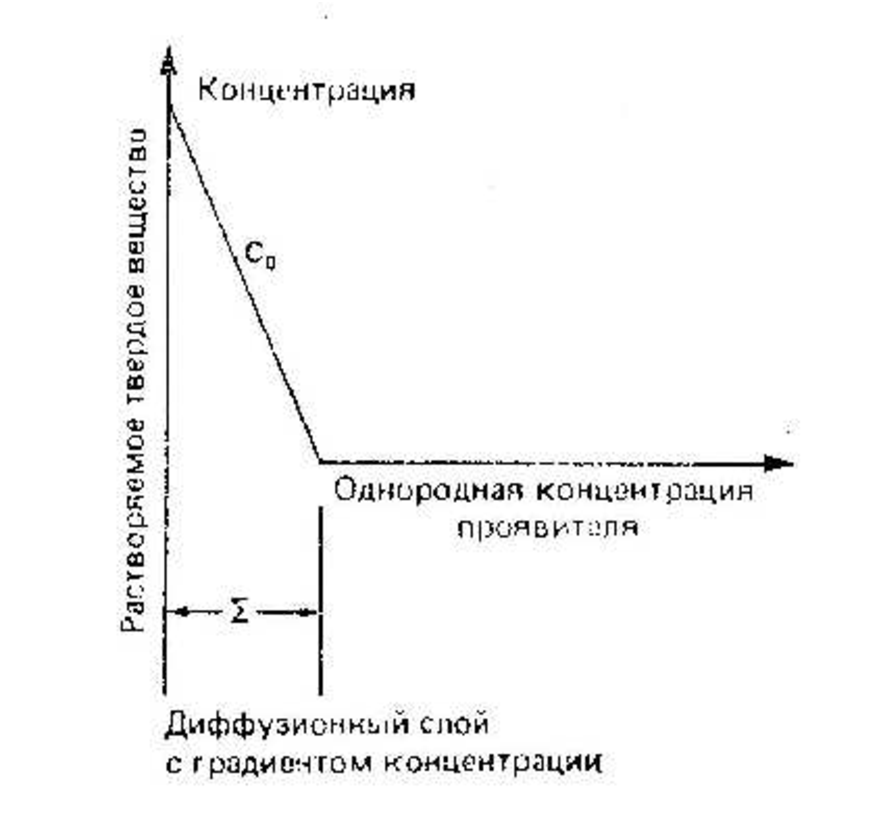
\includegraphics[scale=0.6]{1_5.pdf}
\caption{Градиент концентрации вблизи поверхности проявляемого резиста.}
\label{fig:5}
\end{figure}

Прирост концентрации $dC$ зависит от объема жидкости $V$ и молекулярной массы полимера $М$
\begin{equation}
\frac{dm}{M}\frac{1}{V} \sim dC.
\label{eq:A15}
\end{equation}
Интегрирование уравнения (\ref{eq:A14}) дает
\begin{equation}
\ln\frac{A_s-C}{A_s} = \frac{QSt}{V\Sigma},
\label{eq:A16}
\end{equation}
что эквивалентно реакции первого порядка. Подстановка плотности $р$ и толщины $dz$ в выражение для массы $dm$ или концентрации $dC$ дает экспоненциальную зависимость для скорости растворения
\begin{equation}
\frac{dz}{dt} = A_s MQ \rho Q \exp\left(\frac{-QSt}{MV}\right).
\label{eq:A17}
\end{equation}

Закон Фика, предполагающий, что коэффициент диффузии $Q$ проявителя не зависит от молекулярного веса полимера, не выполняется для многих стекловидных полимеров, в которых набухание препятствует растворению.
В общем случае из закона Фика видно, что скорость растворения полимера обратно пропорциональна его молекулярной массе В резистах наблюдаются два основных типа растворения:
\begin{enumerate}
    \item растворение экспонированного и неэкспонированного резиста практически линейно, если поглощение света или другого вида энергии в пленке однородно по толщине (рисунок~\ref{fig:6}а). Это наблюдается в низко молекулярном ПММА ($М_n<10^4$). При ЭЛ-экспонировании поглощение энергии в тонких пленках (<300 нм) однородно, а в более толстых пленках возрастает с глубиной из-за большего вклада обратного рассеяния. Случай 1 относится к простому послойному растворению пленки.
    \item растворение неэкспонированных участков резиста замедляется в меру длительности индукционного периода (рисунок~\ref{fig:6}6)  Случай 2 учитывает проникновение проявителя в пустоты, но быстрого растворения не происходит из-за образования набухающего гель-слоя или поверхностной адсорбции продуктов растворения. 
\end{enumerate}
\begin{figure}[H]
\center
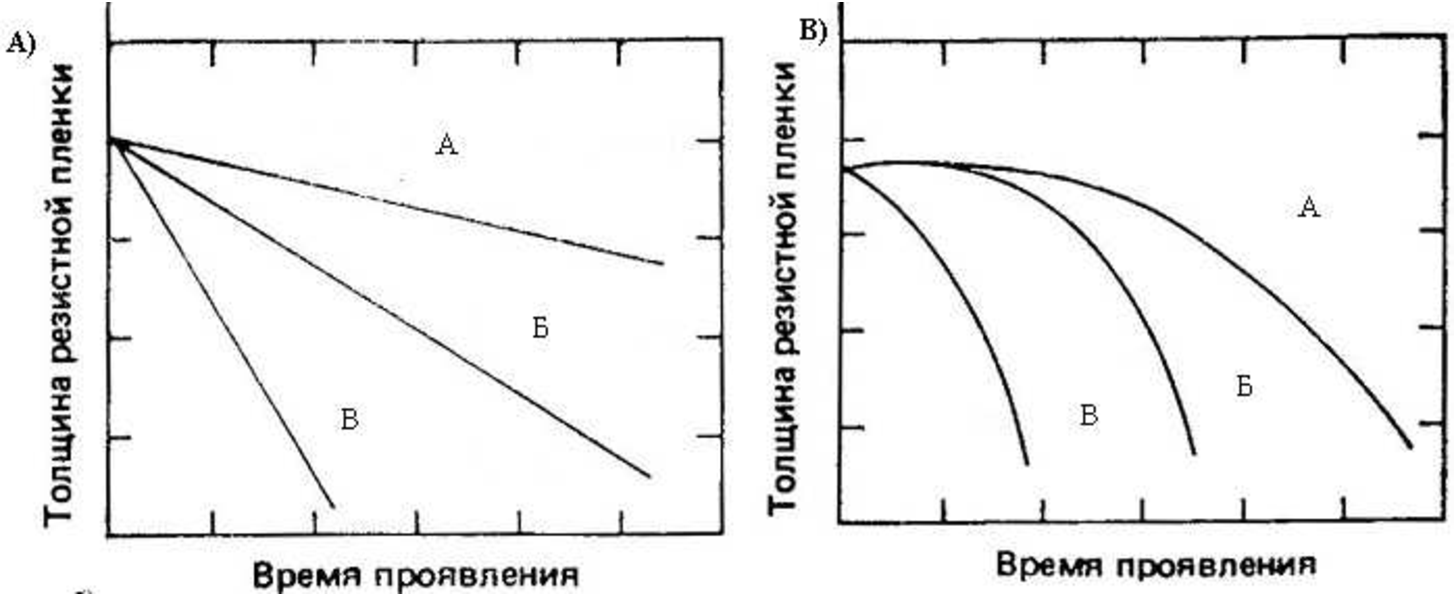
\includegraphics[scale=0.6]{1_6.pdf}
\caption{А) линейно растворяющийся полимер, В) нелинейно растворяющийся резист (индукционный эффект): А~--~неэкспонированный резист, Б~--~экспонированный резист с малой дозой, В~--~экспонированный резист с большой дозой}
\label{fig:6}
\end{figure}

Образование нескольких физических
слоев при растворении поверхности полимера было промоделировано Юберейтером с сотрудниками Растворение может также сопровождаться шелушением или растрескиванием, ослабляющим внутренние напряжения при набухании Образование гель-слоя очень выгодно при наличии индукции, так как растворение неэкспонированного резиста задерживается на несколько минут, в течение которых изображение частично проявляется.

\section{Характеристики резиста}

Для успешного применения резистов на практике, необходимо знание нескольких параметров, называемых еще дозовыми характеристиками. Дозовыми характеристиками электронных резистов являются чувствительность и контрастность. Чувствительность позитивного резиста — это минимальная необходимая для проявления резиста до дна доза экспонирования Чувствительность позитивного резиста характеризует дозу, которую необходимо передать участку этого резиста для его полной проявки за приемлемое время (обычно 1-2 минуты). Чувствительность, как и дозу экспонирования электронного резиста обычно измеряют в $\text{Кл}/\text{см}^2$ . Для
определения чувствительности обычно используют тестовую структуру, состоящую из массива одинаковых элементов (например, квадратов) с
различной дозой экспонирования. Задается определенный шаг дозы от одного элемента к следующему. После экспонирования и проявления тестовой структуры, для позитивного резиста ищут среди проявившихся до дна элементов, тот который был проэкспонирован с минимальной дозой. Эту дозу и принимают равной чувствительности позитивного резиста. В настоящей работе в качестве такой структуры выступает дозовый клин, доза экспонирования которого меняется слева на право в 10 раз.
Другой важной характеристикой электронного резиста является контрастность. Она является характеристикой крутизны рельефа резиста после проявления. В литературе контрастность для позитивного резиста определяют несколькими способами	В качестве контрастности для
позитивного резиста, можно предложить использовать параметр растворимости. Действительно, обратная молекулярная масса полимерного резиста зависит от дозы экспонирования. 
Таким образом, можно записать, что
\begin{equation}
D\approx \frac{1}{M}.
\label{eq:A18}
\end{equation}
Скорость проявления линейного растворяющегося резиста может быть описана степенной зависимостью \cite{16,22,23}
\begin{equation}
v=aM^{-\gamma}.
\label{eq:A19}
\end{equation}
Тогда используя формулы (\ref{eq:A18}) и (\ref{eq:A19}) можно получить зависимость скорости проявления резиста от дозы экспонирования 
\begin{equation}
v=v_0\left(\frac{D}{D_0}\right)^\gamma,
\label{eq:A20}
\end{equation}
где $v$ это скорость проявления области проэкспонированной с дозой $D$, а $v_0$ -- скорость проявления области проэкспонированной с дозой $D_0$. параметр $\gamma$ принимается за контрастность. 
